% ===================================================================
%  Human Brain Mapping — Technical Report
%  Scanner Vendor Harmonisation of Spinal Cord qMRI Biomarkers
% ===================================================================
\documentclass[12pt,a4paper]{article}

% Packages
\usepackage[utf8]{inputenc}
\usepackage[T1]{fontenc}
\usepackage{amsmath,amssymb}
\usepackage{graphicx}
\usepackage{booktabs}
\usepackage[margin=2.5cm]{geometry}
\usepackage{hyperref}
\usepackage{setspace}
\usepackage{caption}
\usepackage{enumitem}
\usepackage{float}
\usepackage{lineno}
\usepackage{multirow}
\usepackage{siunitx}
\usepackage{tabularx}
\usepackage{xurl}
\usepackage{pdflscape}
\setlength{\emergencystretch}{3em}

\hypersetup{colorlinks=true,linkcolor=blue,citecolor=blue,urlcolor=blue}
\onehalfspacing

\begin{document}
\linenumbers

% ===================================================================
% Title and author block (NMR in Biomedicine single-blind review; integrated 2026-09-21)
\begin{center}
{\LARGE\bfseries Scanner Vendor Harmonisation of Spinal Cord Quantitative MRI Biomarkers: A Five-Method Benchmark\par}
\vspace{8mm}

{\large Yilin Zhu\textsuperscript{1} and Dengke Wu\textsuperscript{2,*}\par}
\vspace{4mm}

\textsuperscript{1}Changsha Hospital of Traditional Chinese Medicine (Changsha No.\ 8 Hospital), Changsha, Hunan, China \\
\textsuperscript{2}Department of Emergency Medicine, and Emergency Medicine and Difficult Diseases Institute, The Second Xiangya Hospital of Central South University, Changsha 410011, Hunan, China
\vspace{3mm}

\textsuperscript{*}Corresponding author
\vspace{3mm}

\textbf{Corresponding author:} Dengke Wu, MD \\
Email: \href{mailto:wudk2010@csu.edu.cn}{wudk2010@csu.edu.cn} \\
Tel: +86 731 8529 5000; Fax: +86 731 8529 5001 \\
ORCID: \href{https://orcid.org/0000-0003-4101-8461}{0000-0003-4101-8461}
\vspace{3mm}

\textbf{ORCID:} Yilin Zhu \href{https://orcid.org/0009-0004-2552-9493}{0009-0004-2552-9493}; Dengke Wu \href{https://orcid.org/0000-0003-4101-8461}{0000-0003-4101-8461}
\end{center}

\vspace{6mm}

% ===================================================================
\section*{Abstract}

\noindent\textbf{Objectives:} Quantitative spinal cord MRI biomarkers vary systematically with scanner vendor, which limits multi-centre pooling, yet no harmonisation benchmark exists for spinal cord data. We benchmarked five post-hoc harmonisation methods on the open spine-generic dataset.

\noindent\textbf{Methods:} Eight biomarkers (T2w-CSA, GM-CSA, MTR, MTsat, FA, MD, AD, RD) were extracted from 267 participants scanned at 43 sites on three vendors (site and vendor perfectly nested). ComBat, ComBat-joint, CovBat, RELIEF and a mixed-effects/fixed-effects hybrid (LME/FE) were compared on four pre-specified endpoints---vendor-effect removal, biological-covariate recovery, subject-level preservation, and machine-learnability of the vendor signature---in healthy-control ($N=188$) and pathology-inclusive ($N=246$) complete-case cohorts. Leave-one-vendor-out validation tested generalisation to unseen manufacturers.

\noindent\textbf{Results:} Vendor effects were large at baseline and dwarfed age- and sex-related variance. All methods reduced vendor variance to near zero on the metrics they optimise, but a stricter, leakage-free test---machine detection of vendor from the biomarker profile---showed that a residual vendor signature persists for every method, smallest for CovBat and largest for LME/FE. Harmonisation unmasked age associations in diffusion metrics that were undetectable at baseline, and improved classification of radiological cord-compression labels, an exploratory endpoint that is substantially confounded by age. Methods traded multivariate vendor removal against subject-level preservation along a Pareto frontier. Only ComBat and ComBat-joint generalised to an unseen vendor without significant degradation, and joint estimation degraded least.

\noindent\textbf{Conclusion:} For pooled multi-vendor spinal cord qMRI datasets of comparable structure, ComBat-family harmonisation, joint estimation in particular, may be appropriate as a preprocessing step, provided the residual vendor signature and the site-nested design are reported alongside pooled analyses.

\vspace{4mm}
\noindent\textbf{Key Points:}
\begin{enumerate}[nosep,leftmargin=*]
  \item Scanner vendor effects are the dominant source of variance in multi-centre spinal cord qMRI, exceeding age and sex effects by one to two orders of magnitude, so harmonisation should be considered before pooling.
  \item All five benchmarked methods remove vendor variance on the metrics they optimise, but a stricter machine-learning test shows residual vendor signatures remain, and methods that remove more vendor signal distort individual subjects' data more.
  \item With only three vendors, latent-structure and mixed-effects methods failed to generalise to an unseen vendor; ComBat with joint estimation across biomarkers transferred most stably.
\end{enumerate}

\vspace{4mm}
\noindent\textbf{Keywords:} Spinal cord; Quantitative MRI; Harmonisation; ComBat; Multicentre study; Reproducibility; Scanner vendor effects

\vspace{4mm}
\noindent\textbf{Abbreviations:} AD = axial diffusivity; ComBat = Combatting batch effects; CovBat = Covariance Batch harmonisation; CSA = cross-sectional area; DCM = degenerative cervical myelopathy; FA = fractional anisotropy; HC = healthy control; ICA = independent component analysis; LME/FE = linear mixed-effects / fixed-effects hybrid; LOVO = leave-one-vendor-out; MD = mean diffusivity; MT = magnetisation transfer; MTR = magnetisation transfer ratio; MTsat = magnetisation transfer saturation; PERMANOVA = permutational multivariate analysis of variance; qMRI = quantitative magnetic resonance imaging; RD = radial diffusivity; RELIEF = REmoval of Latent Inter-scanner Effects through Factorization

% ===================================================================
\section{Introduction}

Quantitative MRI (qMRI) biomarkers of the spinal cord---cross-sectional area (CSA), magnetisation transfer ratio (MTR), magnetisation transfer saturation (MTsat), and diffusion tensor metrics (FA, MD, AD, RD)---provide non-invasive windows into atrophy, demyelination, and axonal integrity in multiple sclerosis, degenerative cervical myelopathy, and spinal cord injury [1--3]. Multi-centre consortia are increasingly adopting these biomarkers, but systematic vendor-dependent variability limits cross-site pooling [4,5]. A recent pan-European survey by the European Society of Radiology documented marked heterogeneity in MRI quality assurance and control practices across 37 countries [6], underscoring the urgency of robust harmonisation.

Even under standardised acquisition protocols, differences in gradient hardware, RF coil geometry, and vendor-specific reconstruction pipelines introduce offsets that often exceed the biological effect sizes of interest [4,7]. Statistical post-hoc harmonisation methods (ComBat [8--10], CovBat [11], RELIEF [12], and linear mixed-effects models [13]) have been extensively benchmarked in brain imaging and reviewed in the broader context of multicentre radiomics [14] but remain uncharacterised for spinal cord qMRI. Fortin et al.\ first applied ComBat to multi-site DTI [10], establishing a framework later extended to cortical thickness [9], longitudinal harmonisation [15], covariance harmonisation [11], latent-factor removal [12], and out-of-sample harmonisation for new sites [16]. Middleton et al.\ demonstrated ComBat's effectiveness for spinal cord DTI [17], and Jodoin et al.\ provided deployment guidance for diffusion MRI [18], but no study has systematically compared the full ComBat family across a comprehensive spinal cord biomarker panel using unified multi-endpoint evaluation.

The spinal cord presents distinct harmonisation challenges: small per-site sample sizes in the complete-case analysis sample (HC: median 5 subjects per site, range 2--8; ALL: median 6, range 2--11) challenge empirical Bayes shrinkage; strong inter-metric correlations (diffusion metrics are intrinsically coupled; MTR and MTsat share acquisition-dependent variance) motivate multivariate evaluation; and it has not been quantified how much disease-related variance each method retains while removing vendor effects.

Here we benchmark five methods on eight spinal cord qMRI biomarkers using four complementary endpoints: vendor-effect removal, biological-covariate recovery, subject-level preservation, and machine-learnability of the vendor signature. We extend prior work through: (i) formal comparison of the full ComBat family (including covariance and latent-factor extensions); (ii) multivariate evaluation via PERMANOVA; (iii) a Pareto-frontier analysis of the decontamination--preservation trade-off; and (iv) leave-one-vendor-out external validation to test generalisability.

% ===================================================================
\section{Materials and Methods}

\subsection{Dataset and Cohorts}

The spine-generic multi-subject dataset (release r20231212) [1] comprises 267 subjects scanned at 43 sites across three vendors (GE Healthcare: 37 subjects at 6 sites; Philips: 50 subjects at 8 sites; Siemens Healthineers: 180 subjects at 29 sites) using a standardised consensus protocol [4]; the release used here adds seven subjects and one site to the 260 participants at 42 sites described in the original data descriptor [1]. The dataset composition and the eight-biomarker panel are illustrated in Figure~1a,b. Site and vendor are perfectly nested (each site operates a single scanner from one vendor); reported vendor effects thus represent the composite ``vendor-in-site'' effect. Of the 267 subjects, 21 (7.9\%) were missing at least one biomarker---in almost all cases because a contrast was not acquired at the site rather than because of quality-control exclusions---leaving 246 complete cases; of the 203 healthy controls, 188 were complete cases (missingness mechanisms are itemised in Section~2.8 and Supplementary Material~S1). The complete-case analysis sample comprised 40 sites (GE 5, Philips 8, Siemens 27). Demographics were balanced across vendors in the complete-case analysis sample (Table~1; all $p\geq0.203$).

\begin{table}[H]
\centering
\small
\setlength{\tabcolsep}{4pt}
\caption{Demographic and acquisition characteristics by vendor (HC complete-case analysis sample, $N=188$). Continuous variables: mean $\pm$ SD, one-way ANOVA. Categorical variables: count (\%), $\chi^{2}$ test. Site and vendor are perfectly nested (40 sites across 3 vendors in the analysis sample; 43 sites in the full dataset).}
\label{tab:demographics}
\begin{tabular}{lrrrrr}
\toprule
Characteristic & GE & Philips & Siemens & Total & $p$-value \\
\midrule
$N$ & 25 & 33 & 130 & 188 & --- \\
Sites ($n$) & 5 & 8 & 27 & 40 & --- \\
Subjects per site, median [range] & 5 [2--8] & 4 [2--6] & 5 [2--8] & 5 [2--8] & --- \\
Age, years (mean $\pm$ SD) & 27.0 $\pm$ 4.9 & 27.9 $\pm$ 4.1 & 29.0 $\pm$ 6.0 & 28.5 $\pm$ 5.6 & 0.203 \\
Age range & 19--39 & 23--38 & 20--52 & 19--52 & --- \\
Sex = F & 13 (52.0\%) & 18 (54.5\%) & 60 (46.2\%) & 91 (48.4\%) & 0.640 \\
Sex = M & 12 (48.0\%) & 15 (45.5\%) & 70 (53.8\%) & 97 (51.6\%) & --- \\
Height, cm & 170.1 $\pm$ 8.7 & 171.3 $\pm$ 9.9 & 173.2 $\pm$ 10.1 & 172.5 $\pm$ 9.9 & 0.277 \\
Weight, kg & 66.4 $\pm$ 13.6 & 66.5 $\pm$ 13.6 & 67.9 $\pm$ 13.1 & 67.5 $\pm$ 13.2 & 0.781 \\
Scanner models ($n$) & 3 & 4 & 5 & 12 & --- \\
\bottomrule
\end{tabular}
\end{table}

Two pre-specified cohorts were analysed: HC ($N=188$ complete-case healthy controls) isolates pure vendor-driven variance; ALL ($N=246$ complete-case, including 56 mild cervical compression and 2 DCM) approximates real-world deployment. Pathology distribution was balanced across vendors ($\chi^2\ p=0.661$). The pathology labels shipped in the dataset's \texttt{participants.tsv} are radiological assessments only: two experienced radiologists screened the MRI scans for spinal cord compression and annotated 64 of the 267 subjects, mostly mild compression, without any clinical diagnosis [3]. Mild cervical compression is common with ageing and is not necessarily pathological, and with only two DCM cases the pathology group is essentially radiological mild compression; moreover, the biomarkers were extracted at C2--C3 rather than at the level of compression. All analyses involving these labels (Section~3.3) are therefore exploratory. Detailed cohort flow and missingness patterns are provided in Supplementary Material~S1.

\subsection{Biomarker Extraction and Processing}

Eight biomarkers spanning four acquisition families were extracted using the Spinal Cord Toolbox [19] (Figure~1b): T2w-CSA from T2-weighted structural imaging, MTR and MTsat from magnetisation transfer, and FA, MD, AD and RD from diffusion tensor imaging, all sampled at the C2--C3 level; and GM-CSA from T2\textsuperscript{*}-weighted imaging, averaged over every segmented cervical slice because the T2\textsuperscript{*} acquisition does not span the vertebral levels resolved on T2w.

All segmentations, vertebral labels and metric maps were generated de novo for this study; the manual disc labels and segmentations shipped in the dataset's \texttt{derivatives} were not used, so that every subject was processed by one uniform, fully automatic pipeline. The pipeline follows the spine-generic reference pipeline (\url{https://spine-generic.readthedocs.io}) with four deliberate differences: (i) the seven level-restricted biomarkers were sampled in a common C2--C3 window so that all metrics cover identical anatomy, whereas the reference pipeline samples MTR/MTsat and DTI metrics over C2--C5 and GM-CSA over C3--C4; (ii) spinal cord and grey matter segmentation used the current contrast-agnostic nnUNet models (\texttt{sct\_deepseg spinalcord}; \texttt{sct\_deepseg graymatter}, model release r20250420) rather than the legacy \texttt{sct\_deepseg\_sc}/\texttt{sct\_deepseg\_gm}; (iii) vertebral labelling used \texttt{sct\_label\_vertebrae} on the T2w image in fully automatic mode, without the manual disc labels used by the reference pipeline (the consequences of this choice are audited in Supplementary Material~S2.2); and (iv) MT and diffusion metrics were averaged within the whole-cord mask rather than the PAM50 white-matter atlas. A step-by-step comparison with the reference pipeline is given in Supplementary Material~S2.

Because the installed SCT build (\texttt{7.4.dev0}) does not correspond to a numbered release, we report the exact source snapshot: master branch, git commit \texttt{93923f5e363d9400fbadab07459f125a08b21ad8} (2 June 2026, sixteen commits after the 7.3 release). The complete processing and analysis code is available at \url{https://github.com/wudengke2010/spine-generic-harmonization}.

Missing values arose from absent or incomplete acquisitions and, in three subjects, from the labelled C2--C3 level falling outside the MT field of view; diffusion metrics were unavailable for two of these subjects for the same reason, and for the third because the extracted FA values were identically zero and were set to missing by the aggregation-stage rule detailed in Supplementary Material~S2. No subject was excluded on the basis of a quality-control score (Supplementary Material~S1--S2).

\subsection{Harmonisation Methods}

Five methods were evaluated (full mathematical details in Supplementary Material~S3). In all methods, scanner vendor (GE/Philips/Siemens, three levels) served as the batch variable; because sites are perfectly nested within vendors, vendor-level and site-level offsets are statistically confounded, and the composite ``vendor-in-site'' effect is the harmonisation target:

\textbf{ComBat} [8--10]: Per-metric location-and-scale adjustment with empirical Bayes shrinkage on vendor-specific parameters. Each biomarker harmonised independently.

\textbf{ComBat-joint} [9]: All eight biomarkers harmonised jointly (joint empirical Bayes), preserving cross-metric covariance structure.

\textbf{CovBat} [11]: ComBat-joint followed by principal component (PC) correction---residuals projected onto PCs, each PC harmonised independently, then projected back. PCs explaining at least 95\% of the residual variance were retained: $K=5$ of 8 (cumulative variance 95.9\% in the HC cohort, 95.6\% in the ALL cohort; the first three PCs accounted for 85.6\% and 84.9\%, respectively).

\textbf{RELIEF} [12]: ComBat-joint followed by independent component analysis (ICA) of residuals. Our implementation is a residual-ICA variant of RELIEF (REmoval of Latent Inter-scanner Effects through Factorization), rather than the linked matrix factorisation of the original report; this distinction is revisited in the Limitations. Components with significant vendor association (Benjamini-Hochberg FDR-controlled ANOVA, $q<0.05$) are zeroed. In the present dataset, no component reached significance (all $q\geq0.99$), rendering the pipeline functionally equivalent to ComBat-joint with an additional PCA/ICA round-trip.

\textbf{LME/FE}: Vendor as a random intercept with age and sex fixed effects. When the random-effects covariance matrix was singular (expected with only 3 vendor levels, well below the recommended $k\geq5$ for stable REML estimation), the model fell back to ordinary least squares centring (9 of 16 biomarker$\times$cohort combinations, 56\%; see Results). Only MD and AD achieved stable LME fits in both cohorts. This hybrid is referred to below as LME/FE.

\subsection{Evaluation Endpoints}

Four complementary endpoints were evaluated per method per cohort (detailed in Supplementary Material~S4). Table~2 summarises what each endpoint measures, the desirable direction, and its main caveat.

\textbf{Vendor-effect removal}: Univariate $\eta^2$ (ANOVA), intraclass correlation coefficient (ICC), and multivariate PERMANOVA $R^2$ (Euclidean distance, 9,999 permutations) [20]. All five methods and the unharmonised baseline---including ComBat and LME/FE, which were refitted on the unified complete-case sample---were evaluated on the same subjects, with per-dimension z-scoring of biomarkers before PERMANOVA. Consequently, the multivariate $R^2$ equals the mean of the per-metric $\eta^2$ for every method (a mathematical identity of z-scored Euclidean PERMANOVA), so univariate and multivariate summaries are directly comparable throughout.

\textbf{Biological-covariate recovery}: Type-II semi-partial $R^2$ for age and sex from linear models. Because age and sex are modelled as protected covariates by every method, recovery in the expected direction is guaranteed by construction; the informative quantities are the magnitude recovered and the per-metric significance patterns (Section~3.4).

\textbf{Subject-level preservation}: for each biomarker, Pearson $r$ across subjects between the pre- and post-harmonisation values---that is, preservation of the subject ranking on that biomarker---averaged over the eight biomarkers.

\textbf{Machine-learnability of the vendor signature}: Following the site-detection paradigm of Chen et al.\ [11], a random forest (500 trees, minimum leaf size 5, balanced class weights) was trained to classify scanner manufacturer (Siemens/GE/Philips) from the 8-biomarker profile of each subject, using repeated stratified 5-fold cross-validation (20 repeats). To prevent information leakage, each harmonisation model was refitted on the training folds only and applied to the held-out fold within every cross-validation split. Harmonisation used vendor labels on training and test folds alike, as it would at deployment; the random forest itself never saw vendor labels. The macro one-vs-rest AUC quantifies residual vendor information detectable by machine learning, a stricter criterion than univariate $\eta^2$ because nonlinear combinations of features can encode vendor structure invisible to marginal statistics. As an exploratory sensitivity analysis, the same classifier, again using all eight biomarkers jointly as input features, was applied to the radiological pathology labels (healthy control vs mild compression/DCM, ALL cohort, $N=246$ complete cases) and to sex labels. A shuffled-label permutation reference calibrated the chance level.

\begin{table}[H]
\centering
\small
\setlength{\tabcolsep}{4pt}
\caption{Evaluation endpoints at a glance: what each endpoint measures, which direction is desirable, and its main caveat.}
\label{tab:endpoints}
\begin{tabularx}{\textwidth}{@{}>{\raggedright\arraybackslash}p{3.0cm}>{\raggedright\arraybackslash}X>{\raggedright\arraybackslash}p{2.2cm}>{\raggedright\arraybackslash}X@{}}
\toprule
Endpoint & What it measures & Desirable direction & Main caveat \\
\midrule
Vendor $\eta^2$ / PERMANOVA $R^2$ & Fraction of biomarker variance explained by vendor (univariate / multivariate; identical under z-scoring) & Lower & Every method optimises exactly this criterion, so near-zero values are a process check, not independent validation (chance level $\approx0.011$) \\
Vendor AUC (leakage-free) & Residual vendor signature detectable by a random forest when harmonisation is refit within each fold & Lower (toward 0.50) & Stricter than $\eta^2$; assumes vendor labels are known at deployment \\
Age/sex semi-partial $R^2$ & Biological-covariate variance retained after harmonisation & Higher vs.\ baseline & Age and sex are protected covariates in all methods, so gains are partly by design \\
$r_{\text{pre,post}}$ & Per-biomarker correlation across subjects, pre- vs post-harmonisation (subject-ranking preservation) & Higher & Pooled correlation mixes within- and between-vendor variance; ceiling $\sqrt{1-\eta^2}$ \\
LOVO $\eta^2$ and LOVO/internal ratio & Generalisation to a vendor excluded from training & No increase vs.\ internal & Evaluated on the pooled within-fold sample; unseen-vendor transforms are heuristics (z-score matching / projection) \\
Pathology AUC (exploratory) & Discrimination of radiological cord-compression labels from all eight biomarkers combined & Higher vs.\ baseline & Radiological, not clinical, labels; age-related; not externally validated \\
\bottomrule
\end{tabularx}
\end{table}

\subsection{Leave-One-Vendor-Out External Validation}

For each method, harmonisation models were trained on subjects from two vendors and applied to the held-out third vendor in three rotation folds. Test-vendor transformation used z-score distribution matching (ComBat, ComBat-joint) or projection onto training PCA/ICA space (CovBat, RELIEF). LME/FE assigned offset=0 to unseen vendors. Three of the four endpoints (vendor-effect removal, biological-covariate recovery, and subject-level preservation; machine-learnability and the ALL-cohort pathology/sex classification indices were not re-evaluated) were evaluated after pooling the harmonised training-vendor and held-out test-vendor data within each fold (Supplementary Material~S5). For ComBat, ComBat-joint, and LME/FE, the test-vendor transformation applies a per-biomarker affine (location--scale) map, so the test-vendor pre/post correlation equals 1.0 by construction. For CovBat and RELIEF, in contrast, projection onto the training PCA/ICA basis mixes biomarker dimensions, and the test-vendor pre/post correlation fell below 1 (fold-wise range $r=0.85$--$0.97$ across the three held-out vendors; fold means 0.90 for CovBat and 0.95 for RELIEF). This indicates genuine distortion of held-out-vendor subject rankings.

LOVO preservation statistics for the first group therefore reflect the pooled sample rather than the unseen vendor in isolation. Similarly, the LOVO/internal $\eta^2$ ratio below 1 for ComBat-joint reflects the pooled evaluation sample rather than genuine improvement on unseen vendors.

\subsection{Supplementary Analyses}

Design C reduced-imbalance subsample analysis restricted Siemens to 40 randomly drawn subjects per seed (HC cohort, retaining all GE and Philips subjects; $n\approx98$ per subset; residual vendor imbalance $\max/\min=1.60$ vs.\ $5.2$ in the full analysis; 20 random seeds), with all methods refitted per subset using the same canonical implementations as the main analysis, to isolate the effect of vendor imbalance from method performance. A true-equal-$n$ sensitivity analysis (25 subjects per vendor, $n=75$, imbalance ratio $=1.00$) is reported in Supplementary Material~S6. In addition, because only three vendor levels are available, ComBat was refitted with site (40 levels) or scanner model (12 levels) as the batch variable (Supplementary Material~S10; Section~3.8).

\subsection{Uncertainty Quantification}

Ninety-five per cent confidence intervals for key point estimates were obtained using a stratified nonparametric bootstrap ($B=2{,}000$), resampling subjects with replacement within each scanner-vendor stratum to preserve group proportions. Percentile intervals are reported for $r_{\text{pre,post}}$ and for the baseline vendor effect size. Because marginal CIs for $r_{\text{pre,post}}$ overlap across methods, method pairs were additionally compared with a within-resample paired bootstrap: for each bootstrap sample, all methods' $r$ values were recomputed and their differences tested against zero, which removes between-resample variance and directly targets the pairwise contrast. Bootstrap intervals are not reported for post-harmonisation $\eta^2$ or PERMANOVA $R^2$ because harmonisation methods optimise on the same data, rendering subject-level resampling intervals unreliable for these near-degenerate statistics.

\subsection{Reporting Guidelines and Missing Data}

This study follows STROBE reporting guidance for cross-sectional studies where applicable. Subjects with missing biomarker data were excluded via complete-case analysis (HC: $N=188/203$, 7.4\%; ALL: $N=246/267$, 7.9\%). Missingness was driven by site-level acquisition differences---two sites contributed no MT acquisition for any of their subjects, and one site was affected in every subject---and incomplete subjects were older than complete subjects (median 34.0 vs.\ 28.5 years, $p=0.015$) though not different in sex ($p=0.880$). The mechanism was therefore not missing completely at random; the attribution of all 21 incomplete subjects is itemised in Supplementary Material~S1. A separate vertebral-labelling defect affecting 15 HC subjects is documented with a sensitivity analysis in Supplementary Material~S2.

% ===================================================================
\section{Results}

\subsection{Baseline Vendor Effects}

At baseline, vendor explained 31\% of univariate biomarker variance (mean $\eta^2=0.315$, 95\% CI [0.273, 0.381], stratified bootstrap; range 0.05--0.70 across metrics) and 31\% of multivariate structure (PERMANOVA $R^2=0.315$, $p=1\times10^{-4}$, the permutation lower bound with 9,999 permutations; HC cohort). These effects exceeded age-related variance by approximately two orders of magnitude and sex-related variance by one order. AD showed the largest vendor effect ($\eta^2_{\text{HC}}=0.70$), followed by MD ($0.46$) and MTsat ($0.34$); among structural metrics, GM-CSA showed the strongest vendor discrepancy ($\eta^2=0.18$, Philips scanners systematically lower; Supplementary Fig.~S3). In the ALL cohort, baseline vendor effects were comparable or larger ($\eta^2=0.336$; PERMANOVA $R^2=0.336$). In summary, vendor affiliation is the dominant source of biomarker variance at baseline, exceeding age-related variance by approximately two orders of magnitude.

\begin{figure}[H]
\centering
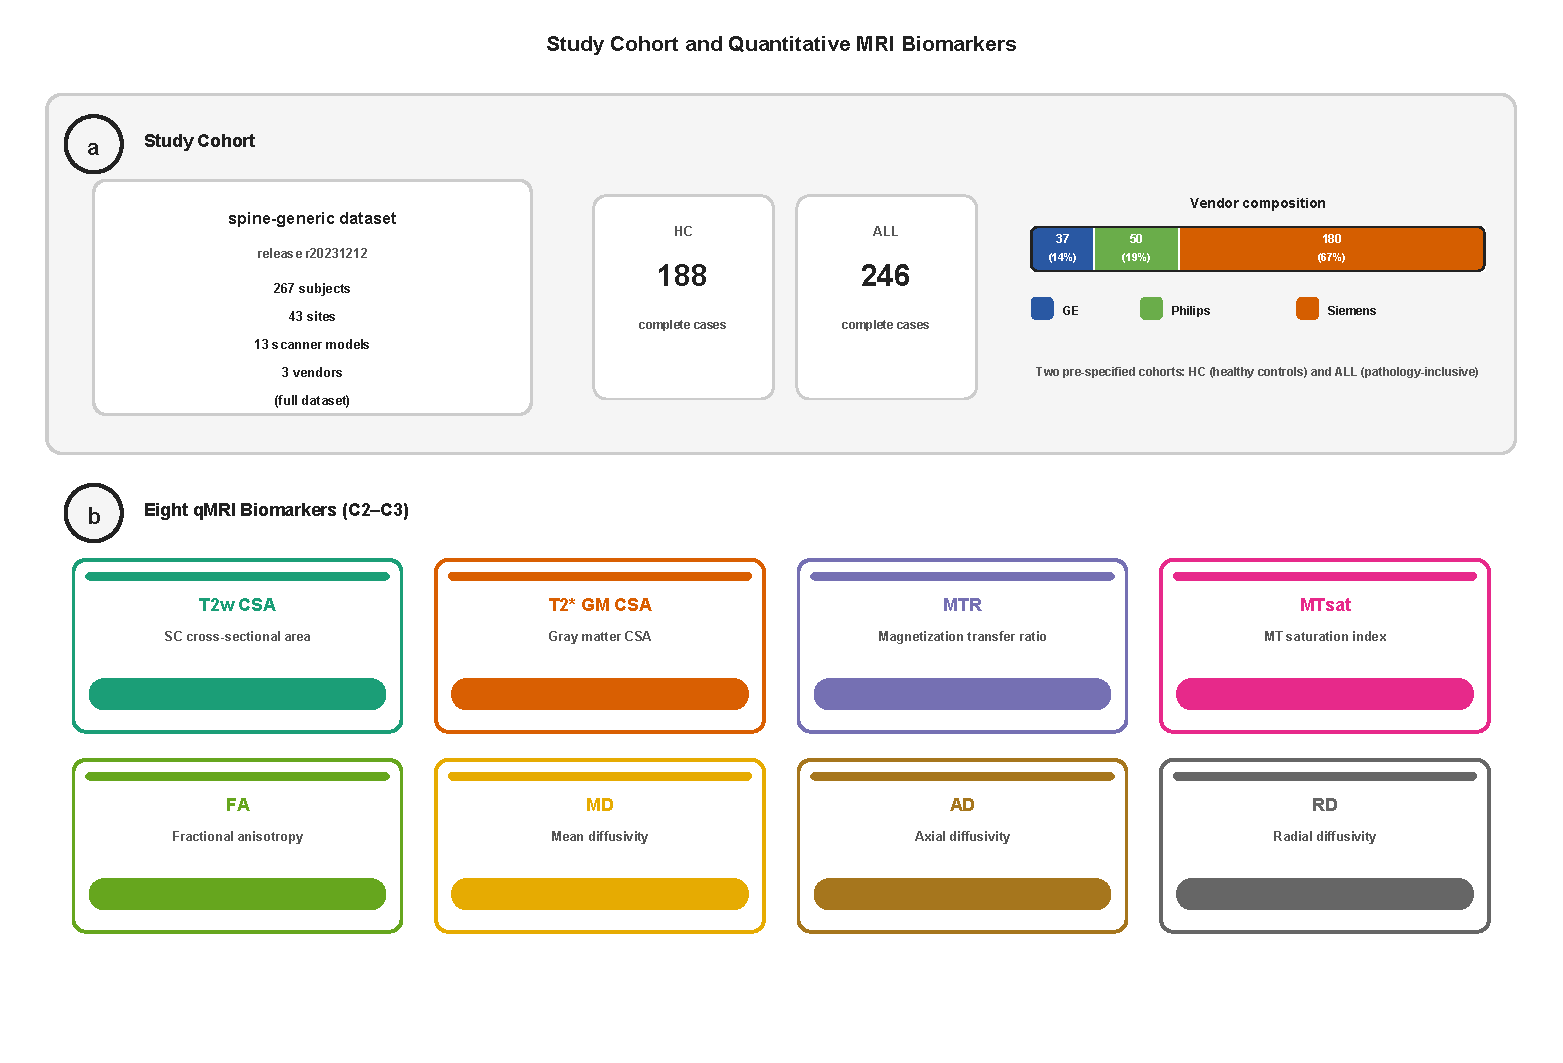
\includegraphics[width=\textwidth]{figures/Fig1.pdf}
\caption{Overview of the study dataset and biomarker panel. \textbf{(a)} Study cohort: the spine-generic multi-subject dataset (release r20231212) [1] comprising 267 subjects scanned at 43 sites on 13 scanner models from three vendors (GE: 37 subjects at 6 sites; Philips: 50 at 8; Siemens: 180 at 29), with the two pre-specified analysis cohorts (HC, $N=188$ complete cases; ALL, $N=246$ complete cases). \textbf{(b)} The eight quantitative MRI biomarkers, spanning four acquisition families. T2w cross-sectional area (T2w-CSA) from T2-weighted structural imaging, magnetisation transfer ratio (MTR) and saturation (MTsat), and fractional anisotropy (FA), mean (MD), axial (AD) and radial (RD) diffusivity from diffusion tensor imaging were sampled at the C2--C3 level; grey matter CSA (GM-CSA) from T2\textsuperscript{*}-weighted imaging was averaged over every segmented cervical slice.}
\label{fig:baseline}
\end{figure}

\subsection{Vendor-Effect Removal}

All five methods reduced vendor $\eta^2$ to between $2.5\times10^{-4}$ (CovBat, HC) and $7.9\times10^{-4}$ (LME/FE, HC; mean $4.8\times10^{-4}$ across methods; Figure~2a,b, Table~3), corresponding to a 400- to 1,240-fold reduction from the baseline mean of 0.315 (mean $\approx2.8$ orders of magnitude across methods). For reference, the $\eta^2$ expected under the null hypothesis of no vendor effect is $(k-1)/(N-1)=2/187\approx0.011$; post-harmonisation values lie far below this chance level, so the effective reduction relative to chance expectation is 92.6--97.6\% across methods (LME/FE lowest at 92.6\%, CovBat highest at 97.6\%). Multivariate vendor structure became indistinguishable from chance (all PERMANOVA $p=1.0$ in both cohorts). These near-zero values should, however, be read as a process check rather than an independent validation: vendor is the harmonisation batch variable, and each method explicitly removes vendor location and scale, so a correctly implemented pipeline is expected to drive $\eta^2$ toward zero by construction. Machine-learnability (below) provides the stricter, non-degenerate criterion.

Covariance structure was displaced from the original to a comparable degree by all methods (Supplementary Fig.~S4). Expressed relative to the total Frobenius norm of the original cross-metric correlation matrix ($\|R_{\mathrm{orig}}\|_F=4.08$ in HC, $4.07$ in ALL), post-harmonisation correlation matrices lay 38.1--41.3\% away from the original in the HC cohort (ComBat 38.1\%, LME/FE 38.3\%, ComBat-joint 38.4\%, RELIEF 40.3\%, CovBat 41.3\%) and 40.2--43.0\% away in ALL (ComBat 40.2\%, ComBat-joint 40.5\%, LME/FE 40.6\%, RELIEF 42.3\%, CovBat 43.0\%). No method therefore preserved the covariance structure in absolute terms. Between-method distances were smaller but far from uniform across the ten method pairs: they ranged from 0.048 (ComBat vs.\ ComBat-joint) to 0.501 (CovBat vs.\ LME/FE) in HC and from 0.036 to 0.479 in ALL, against a mean method-to-original displacement of 1.60 (HC) and 1.68 (ALL). ComBat and ComBat-joint yielded near-identical correlation matrices (0.048 in HC, 0.036 in ALL), as did CovBat and RELIEF (0.094 and 0.078); the remaining eight pairs lay between 0.30 and 0.50. The location--scale methods remained marginally closer to the original than the covariance-projection methods. In summary, every method drives vendor variance far below chance expectation---a process check rather than independent validation---while displacing the original cross-metric covariance structure by 38--43\%.

\begin{figure}[H]
\centering
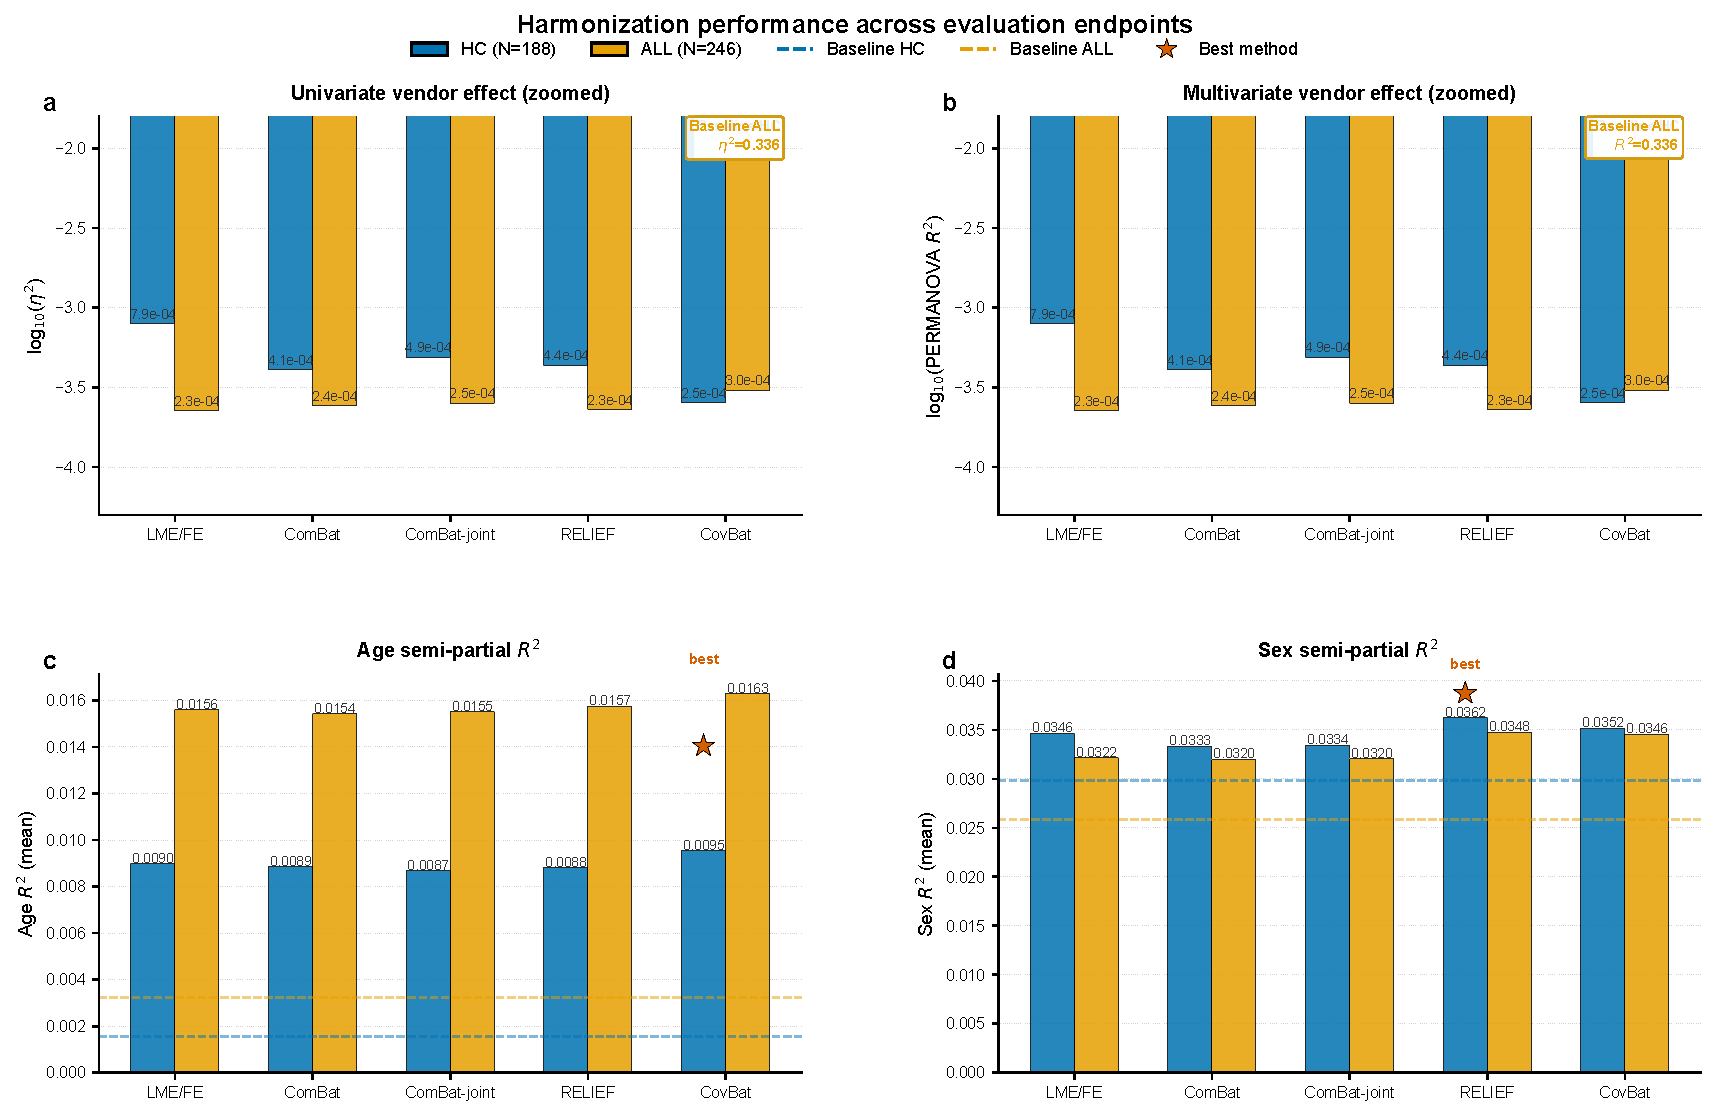
\includegraphics[width=\textwidth]{figures/Fig2.pdf}
\caption{Harmonisation performance by method and endpoint (healthy control cohort; the baseline row shows the Original, unharmonised data). \textbf{(a)} Vendor effect size ($\eta^2$, eta-squared from one-way ANOVA) before and after harmonisation, shown on logarithmic scale. \textbf{(b)} Multivariate vendor structure (PERMANOVA $R^2$, permutational multivariate analysis of variance) on logarithmic scale. \textbf{(c)} Age-related biological signal (semi-partial $R^2$) before and after harmonisation. \textbf{(d)} Sex-related biological signal (semi-partial $R^2$) before and after harmonisation.}
\label{fig:performance}
\end{figure}

\begin{table}[H]
\centering
\scriptsize
\setlength{\tabcolsep}{2.5pt}
\caption{Harmonisation performance summary (HC cohort, complete-case $N=188$). All methods were fitted and evaluated on the same unified complete-case sample. Values are means across 8 biomarkers. $\eta^2_{\text{vendor}}$: post-harmonisation vendor ANOVA effect size; $R^2_{\text{PERMANOVA}}$: multivariate vendor structure (equals the mean per-metric $\eta^2$ by the z-score Euclidean identity); $r_{\text{pre,post}}$: subject-ranking preservation; Age $R^2$: semi-partial age variance explained. LOVO columns show leave-one-vendor-out external validation (PERMANOVA $R^2$ with z-scored Euclidean distance on the pooled within-fold sample, mean across 3 held-out-vendor folds); LOVO ratio: LOVO $\eta^2$ relative to internal $\eta^2$. Values in parentheses are 95\% percentile bootstrap CIs ($B=2{,}000$, stratified by vendor).}
\label{tab:results}
\begin{tabular}{lSSlSSS}
\toprule
Method & {$\eta^2_{\text{vendor}}$} & {$R^2_{\text{PERMANOVA}}$} & {$r_{\text{pre,post}}$ (95\% CI)} & {Age $R^2$} & {LOVO $\eta^2$} & {LOVO ratio} \\
\midrule
Original (baseline) & 3.15e-01 & 0.315 & 1.000 & 0.002 & {---} & {---} \\
ComBat & 4.09e-04 & 0.0004 & 0.789 (0.741--0.825) & 0.009 & 2.46e-03 & 6.0$\times$ \\
ComBat-joint & 4.91e-04 & 0.0005 & 0.806 (0.760--0.839) & 0.009 & 4.42e-04 & 0.9$\times$ \\
CovBat & 2.54e-04 & 0.0003 & 0.782 (0.735--0.816) & 0.010 & 1.01e-03 & 4.0$\times$ \\
RELIEF & 4.36e-04 & 0.0004 & 0.791 (0.743--0.824) & 0.009 & 1.87e-01 & 428$\times$ \\
LME/FE & 7.93e-04 & 0.0008 & 0.816 (0.771--0.848) & 0.009 & 2.01e-01 & 253$\times$ \\
\bottomrule
\end{tabular}
\end{table}

\subsection{Machine-Learnability of the Vendor Signature}

Unharmonised biomarker profiles allowed near-perfect machine detection of scanner manufacturer (macro one-vs-rest AUC $=0.986\pm0.002$ in the ALL cohort; $0.983\pm0.002$ in HC), confirming that the vendor signature dominates the multivariate feature space. After harmonisation refitted within each cross-validation fold to prevent leakage of harmonisation parameters (Methods), detectability decreased substantially but remained above chance for every method (permutation reference $0.495\pm0.038$): CovBat $0.629\pm0.020$, RELIEF $0.690\pm0.017$, ComBat-joint $0.704\pm0.018$, ComBat $0.706\pm0.016$, and LME/FE $0.811\pm0.015$ (ALL cohort, $N=246$; HC values were concordant: 0.670, 0.733, 0.756, 0.751, and 0.851, respectively). Expressed against the chance-adjusted detectability margin, location--scale harmonisation removed 36\% (LME/FE) to 73\% (CovBat) of the machine-detectable vendor information; the method ordering parallels correction depth, the FE fallback being a pure location shift without scale adjustment. Per-vendor detectability after ComBat ranged from 0.67 (Philips) to 0.80 (GE) (Supplementary Table~S8). Complementarily, classification of the exploratory radiological pathology labels (all eight biomarkers combined as input features; Methods) improved from AUC $0.520\pm0.024$ (unharmonised) to $0.582$--$0.625$ across methods (ComBat highest, $0.625\pm0.018$; point AUC 0.64, 95\% CI 0.55--0.72): within-resample paired comparison against Original gave mean $\Delta$AUC $+0.105$, significant for all five methods ($p<0.001$, paired $t$ and Wilcoxon tests). The unpaired Hanley--McNeil test on point AUCs did not reach significance ($p=0.07$), reflecting the power gained by fold-level pairing. Two caveats bound the interpretation of this endpoint. First, the labels are radiological assessments of mostly mild cord compression rather than clinical diagnoses (Section~2.1). Second, the labelled group is substantially older than controls (median 34.0 vs.\ 28.0 years, $p=2\times10^{-7}$), and age alone discriminates the labels (AUC $=0.73$), above any biomarker-based classifier. To test whether the post-harmonisation improvement merely reflects this age confounding, we repeated the classification after residualising every biomarker on age and sex: the improvement persisted (Original $0.565\pm0.027$, ComBat $0.655\pm0.021$; Supplementary Material~S9), indicating that harmonisation unmasks biomarker variance associated with the radiological label beyond age and sex. Sex classification remained stable ($0.646$--$0.670$), indicating that harmonisation removed vendor confounding without distorting this biological signal. In summary, harmonisation removes most, but not all, of the machine-detectable vendor signature, and the method ordering by residual detectability parallels correction depth.

\subsection{Biological-Covariate Recovery}

Before harmonisation, no biomarker showed a significant age association in either cohort (HC: all $p\geq0.34$; ALL: all $p\geq0.19$). After harmonisation, significant age associations emerged selectively in the diffusion metrics: MD and AD in both cohorts (all methods; HC $p=0.006$--$0.049$, ALL $p\leq0.0019$) and additionally RD in ALL ($p\leq0.007$); structural and magnetisation-transfer metrics remained non-significant (all $p\geq0.18$). In mean terms, age $R^2$ increased 5.6--6.2-fold in HC (from $1.5\times10^{-3}$ to $8.7\times10^{-3}$--$9.5\times10^{-3}$) and 4.8--5.0-fold in ALL (from $3.2\times10^{-3}$ to $1.5\times10^{-2}$--$1.6\times10^{-2}$); these fold changes should be read alongside the absolute values and the per-metric significance above, since a ratio of two near-zero variances is itself unstable. Sex $R^2$ showed a similar pattern (1.1--1.3-fold increase). Absolute age effects were larger in ALL, consistent with greater biological heterogeneity, but remained below 2\% of variance. In summary, harmonisation selectively unmasks age associations in the diffusion metrics that vendor variance had obscured at baseline.

\subsection{Subject-Level Preservation and the Pareto Frontier}

Methods diverged on subject-ranking preservation (HC cohort, mean $r$ across methods: LME/FE $=0.816$, ComBat-joint $=0.806$, RELIEF $=0.791$, ComBat $=0.789$, CovBat $=0.782$). This ranking was highly concordant between cohorts (Spearman $\rho=0.90$), with a single adjacent exchange of ranks (ComBat and RELIEF swapped ranks 3--4; ALL values: LME/FE 0.801, ComBat-joint 0.787, ComBat 0.774, RELIEF 0.772, CovBat 0.763). Although the marginal bootstrap 95\% CIs for $r_{\text{pre,post}}$ overlap across methods (Table~3), a within-resample paired bootstrap ($B=2{,}000$) confirmed that the preservation hierarchy is statistically reliable: 8 of 10 method pairs were significantly separated in HC (all $p\leq0.003$) and 9 of 10 in ALL, with LME/FE significantly highest and CovBat significantly lowest (the only non-separated pairs were ComBat vs.\ CovBat and ComBat vs.\ RELIEF in HC, and ComBat vs.\ RELIEF in ALL; Supplementary Table~S7).

In the HC cohort, a Pareto frontier emerged, with methods trading greater multivariate decontamination for lesser subject-level preservation (Figure~3). Because post-harmonisation PERMANOVA $R^2$ values are near-degenerate (Section~3.2), we repeated the frontier ordering using leakage-free vendor detectability (Section~3.3) as the decontamination axis: the corner solutions were preserved (CovBat: maximal removal; LME/FE: maximal preservation), and ComBat and ComBat-joint were indistinguishable on removal in HC (0.751 vs.\ 0.756, within cross-validation noise) with ComBat-joint showing higher preservation (0.806 vs.\ 0.789); in the pathology-inclusive cohort, ComBat-joint weakly dominated ComBat on both axes (lower detectability, 0.704 vs.\ 0.706, and higher preservation, 0.787 vs.\ 0.774), although the removal difference again lies within cross-validation noise. LME/FE's top rank partly reflects its minimal correction: the FE fallback applies a pure location shift without scale adjustment, leaving subject-level variance essentially untouched.

Under the reduced-imbalance subsample (Design C, $n\approx98$ per seed, imbalance ratio $1.60$ vs.\ $5.2$ in the full analysis), the pooled-$r$ preservation hierarchy was retained (LME/FE $r=0.779\pm0.011$, ComBat-joint $0.773\pm0.014$, RELIEF $0.760\pm0.015$, CovBat $0.749\pm0.016$, ComBat $0.745\pm0.015$). The only rank change was the adjacent exchange of ComBat and CovBat, a pair not significantly separated in the main analysis. A true-equal-$n$ sensitivity analysis (25 subjects per vendor, $n=75$, ratio $1.00$) gave concordant results (LME/FE $0.772\pm0.015$; ComBat-family $0.732$--$0.768$).

Absolute values were lower than in the full cohort ($0.782$--$0.816$) because both subsample designs carried a higher baseline vendor-variance fraction: the measured baseline $\eta^2$ was $0.374$ (range $0.343$--$0.401$ across seeds) under reduced imbalance and $0.389$ (range $0.337$--$0.431$) under exact balance, versus $0.315$ in the full analysis. Because pooled $r$ after a location--scale correction cannot exceed $\sqrt{1-\eta^2}$, these baselines imply ceilings of approximately $0.79$ and $0.78$, respectively; every per-method mean fell below its design's ceiling, and the per-seed LME/FE estimate never exceeded the per-seed ceiling in any of the 20 seeds of either design (Supplementary Material~S6). Within-vendor subject rankings were nonetheless preserved near-perfectly by every method in both subsample designs (mean within-vendor $r\geq0.97$), indicating that the pooled-$r$ gradient reflects differential removal of between-vendor variance rather than degradation of within-vendor subject rankings (Supplementary Material~S6). The preservation hierarchy therefore persists under reduced imbalance and under exact balance, indicating that it tracks correction depth rather than the dataset's vendor imbalance; the Pareto frontier nonetheless remains a descriptive characterisation of this dataset's structure.

\begin{figure}[H]
\centering
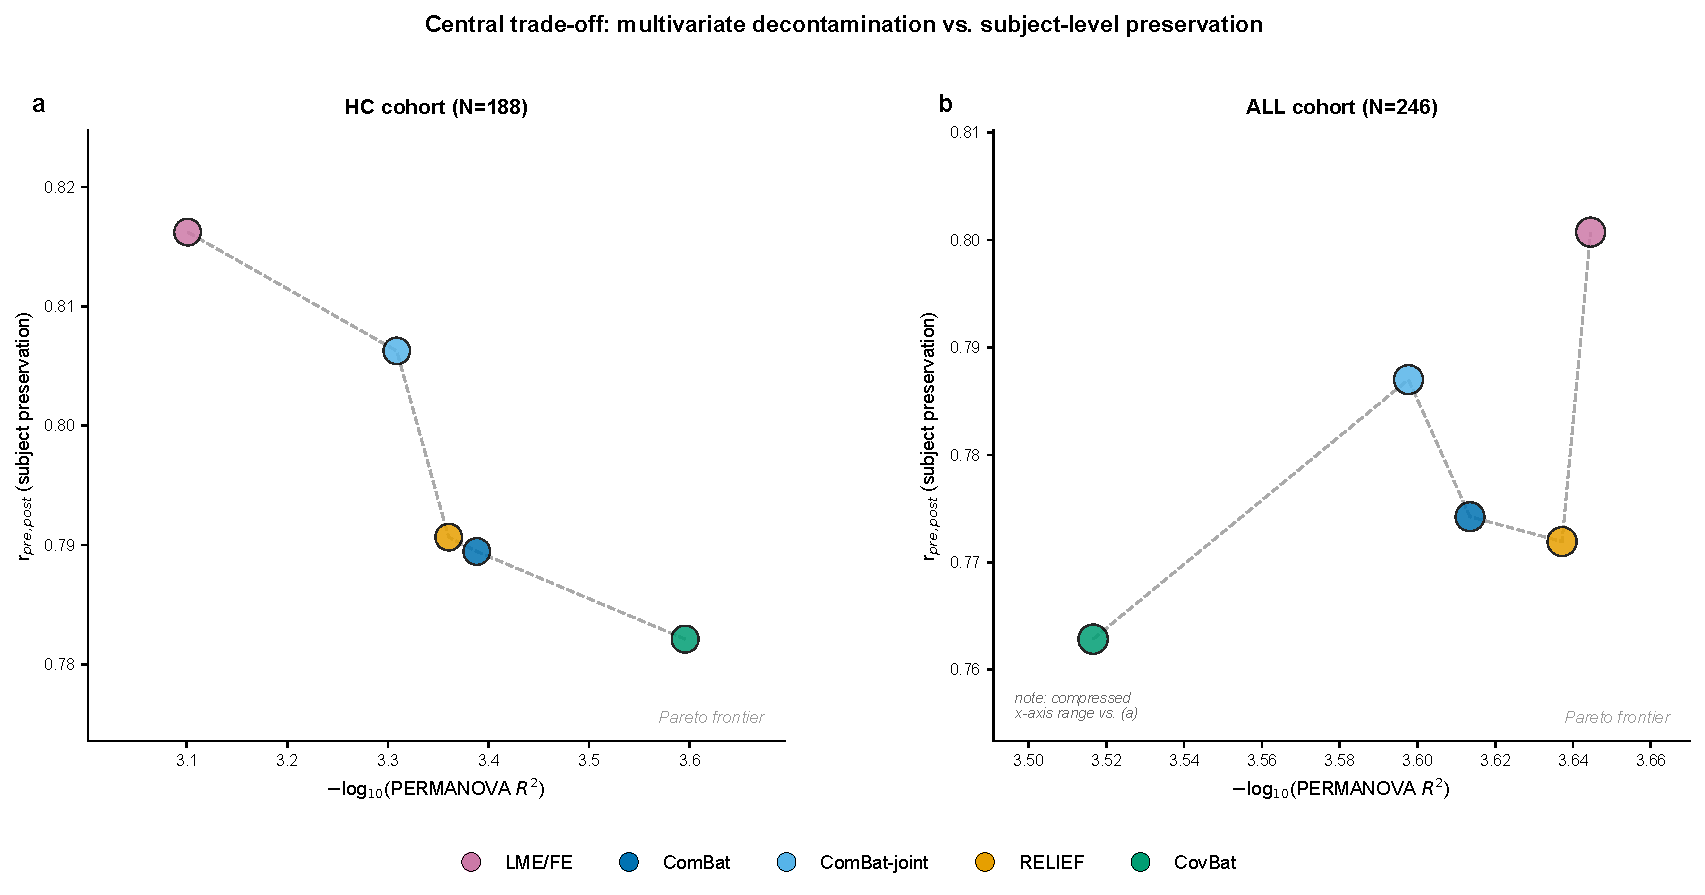
\includegraphics[width=\textwidth]{figures/Fig3.pdf}
\caption{Pareto frontier showing the trade-off between multivariate vendor-effect removal (PERMANOVA $R^2$, permutational multivariate analysis of variance) and subject-level preservation (Pearson correlation $r_{\text{pre,post}}$ between pre- and post-harmonisation biomarker vectors). \textbf{(a)} Healthy control cohort ($N=188$); \textbf{(b)} pathology-inclusive cohort ($N=246$). A monotone frontier is present in the HC cohort; in the pathology-inclusive cohort the ordering is non-monotone (Section~3.5). Each point represents one harmonisation method. Lower right indicates maximal vendor-effect removal; upper left indicates maximal subject-level preservation. The $x$-axis range in \textbf{(b)} is compressed relative to \textbf{(a)} (flagged in the panel), so the apparent spread of methods on this axis should not be compared directly between panels.}
\label{fig:pareto}
\end{figure}

\subsection{LOVO External Validation}

ComBat and ComBat-joint generalised to unseen manufacturers without significant degradation (PERMANOVA $p\geq0.97$ and $p=1.0$ across the three folds, respectively), although ComBat's point estimate rose to LOVO $\eta^2=2.5\times10^{-3}$ (LOVO/internal ratio 6.0), reflecting estimation on the pooled within-fold sample; ComBat-joint remained at $4.4\times10^{-4}$ (ratio 0.9). CovBat showed moderate degradation ($\eta^2=1.0\times10^{-3}$, ratio 4.0). RELIEF and LME/FE failed external validation ($\eta^2_{\text{LOVO}}$: 0.19 and 0.20; PERMANOVA $p<0.01$ in all folds; ratios 428 and 253; Figure~4a--d). This pattern is explained by structural constraints: RELIEF's ICA unmixing matrix is non-transferable across vendor sets, and LME/FE cannot estimate offsets for unseen vendors. CovBat and RELIEF, the two methods that project the held-out vendor onto the training PCA/ICA basis, showed test-vendor pre/post correlations below 1 (fold-wise range $r=0.85$--$0.97$; fold means 0.90 for CovBat and 0.95 for RELIEF). The affine z-score methods, by contrast, preserved held-out-vendor subject rankings exactly by construction.

\begin{figure}[H]
\centering
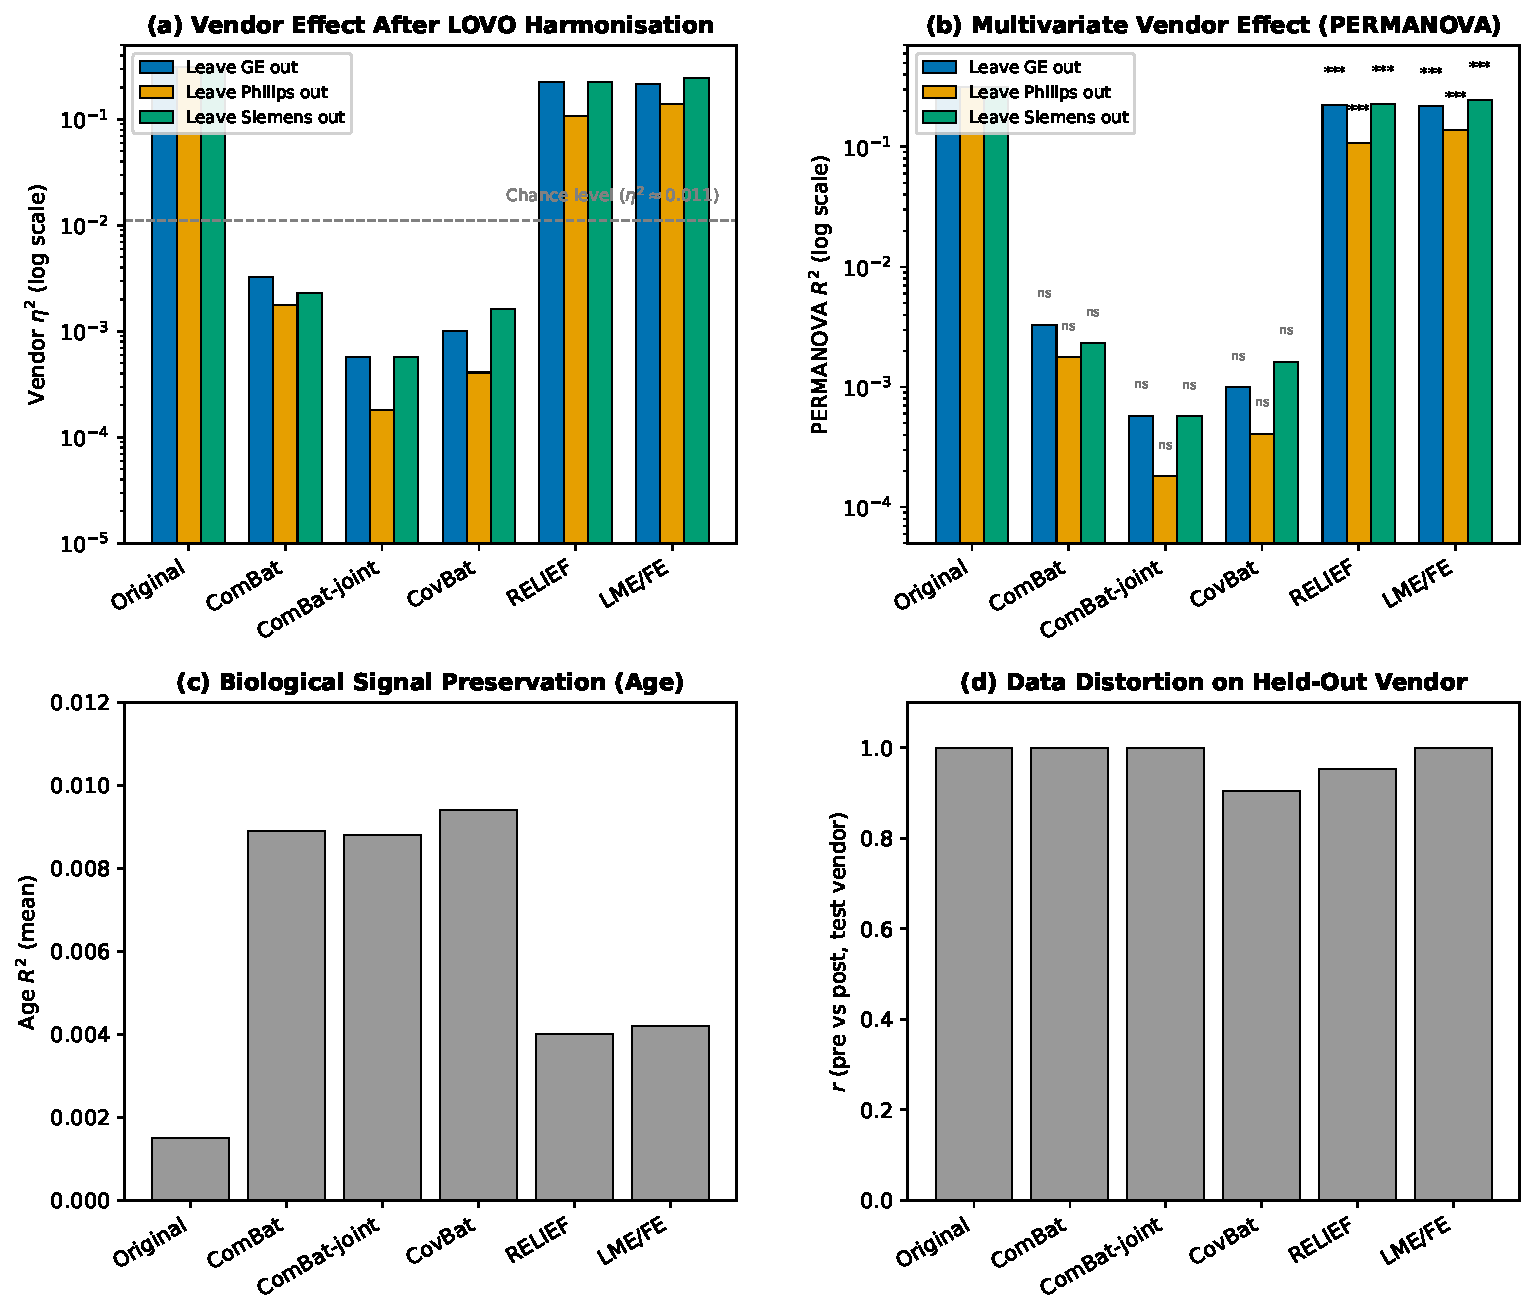
\includegraphics[width=\textwidth]{figures/Fig4.pdf}
\caption{Leave-one-vendor-out (LOVO) external validation. \textbf{(a)} Vendor effect size ($\eta^2$, eta-squared from one-way ANOVA) by method and held-out vendor, shown on logarithmic scale. \textbf{(b)} Multivariate vendor structure (PERMANOVA $R^2$, permutational multivariate analysis of variance) with significance indicators (asterisks denote *$p<0.05$, **$p<0.01$, ***$p<0.001$; ns = not significant). \textbf{(c)} Age-related biological signal (semi-partial $R^2$) recovery. \textbf{(d)} Subject-level preservation (Pearson $r_{\text{pre,post}}$) on unseen vendors. PERMANOVA $R^2$ equals the mean per-metric $\eta^2$ under the z-scored Euclidean distance (Methods), so panels (a) and (b) are numerically identical except for the significance annotation. For the unharmonised baseline (Original) no transformation is fitted, so its pooled within-fold $R^2$ ($0.315$) is identical across folds by construction.}
\label{fig:lovo}
\end{figure}

\subsection{Structural Constraints}

Three methodological observations converge on a single structural limitation of the dataset: only 3 vendors, with sites perfectly nested (43 sites in the dataset, 40 in the analysis sample). The LME random-effects covariance matrix was singular in 56\% of cases because 3 vendor levels provide insufficient information for stable REML variance-component estimation ($k\geq5$ recommended; Table~4). RELIEF's ICA found no vendor-associated components because ComBat-joint preprocessing had already removed vendor mean/scale effects, leaving insufficient residual vendor structure for ICA to detect. These constraints are inherent to the retrospective design; they do not invalidate the internal benchmark findings but bound their generalisability to similarly structured consortia.\begin{table}[H]
\centering
\caption{LME convergence status by biomarker and cohort (complete-case unified fits). FE = fixed-effects fallback (singular random-effects covariance matrix); LME = converged linear mixed-effects model. LME converged in 7 of 16 combinations (44\%); only MD and AD achieved stable LME fits in both cohorts. All 9 FE-fallback cases produced post-harmonisation $\eta^2$ reductions exceeding 99\%, confirming that FE centring is sufficient for vendor-effect removal even when REML fails. The single converged-LME outlier (HC, T2w-CSA; post $\eta^2=4.2\times10^{-3}$) reflects an unstable variance-component estimate rather than FE fallback.}
\label{tab:lme}
\begin{tabular}{llSSSl}
\toprule
Cohort & Biomarker & {$N$} & {$\eta^2$ (pre)} & {$\eta^2$ (post)} & Status \\
\midrule
\multirow{8}{*}{HC} 
  & T2w-CSA   & 188 & 0.0530 & 4.19e-03 & \textbf{LME} \\
  & GM-CSA    & 188 & 0.1761 & 5.09e-04 & FE \\
  & MTR       & 188 & 0.2052 & 1.01e-04 & FE \\
  & MTsat     & 188 & 0.3353 & 4.78e-05 & FE \\
  & FA        & 188 & 0.2902 & 1.28e-04 & FE \\
  & MD        & 188 & 0.4646 & 3.21e-04 & \textbf{LME} \\
  & AD        & 188 & 0.7003 & 5.33e-04 & \textbf{LME} \\
  & RD        & 188 & 0.2927 & 5.07e-04 & FE \\
\midrule
\multirow{8}{*}{ALL} 
  & T2w-CSA   & 246 & 0.0441 & 3.65e-05 & FE \\
  & GM-CSA    & 246 & 0.1673 & 2.06e-05 & FE \\
  & MTR       & 246 & 0.2428 & 2.07e-05 & FE \\
  & MTsat     & 246 & 0.3596 & 1.53e-04 & \textbf{LME} \\
  & FA        & 246 & 0.3116 & 3.55e-04 & \textbf{LME} \\
  & MD        & 246 & 0.5064 & 2.88e-04 & \textbf{LME} \\
  & AD        & 246 & 0.7362 & 4.68e-04 & \textbf{LME} \\
  & RD        & 246 & 0.3199 & 4.72e-04 & FE \\
\bottomrule
\end{tabular}
\end{table}

\subsection{Site- and Scanner-Model-Level Harmonisation}

Because only three vendor levels are available, we additionally refitted per-metric ComBat (empirical Bayes shrinkage) in the HC cohort using site (40 levels) or scanner model (12 levels) as the batch variable (Supplementary Material~S10). Site-level harmonisation reduced the residual vendor effect to the chance level ($\eta^2=0.012$, vs.\ the chance expectation of $\approx0.011$; site-level $\eta^2$ fell from $0.54$ to $0.045$) and recovered slightly more age-related variance (semi-partial $R^2=0.011$ vs.\ $0.009$ for vendor-batch ComBat), at the cost of lower subject-level preservation ($r=0.703$ vs.\ $0.789$). Scanner-model harmonisation was intermediate (vendor $\eta^2=0.0022$; $r=0.763$). Thus finer-grained batch definitions remain viable when the vendor count is small, but they neither resolve the vendor--site nesting nor transfer to unseen vendors or sites, and they cost more subject-level distortion per unit of vendor removal.

% ===================================================================
\section{Discussion}

This study provides, to our knowledge, the first systematic benchmark of statistical harmonisation methods for multi-vendor spinal cord qMRI biomarkers. Six principal findings emerge.

First, baseline vendor effects in spinal cord qMRI are large ($\eta^2=0.31$, PERMANOVA $R^2=0.315$), comparable to or exceeding brain imaging reports [9--11] and dominating biological variation by approximately two orders of magnitude. In absolute terms, the observed baseline corresponds to ~31\% of cross-biomarker variance attributable to vendor. This suggests that vendor offsets, if uncontrolled, would confound biomarker contrasts across vendors in any pooled analysis. Physical harmonisation, such as vendor-specific recalibration of magnetisation transfer metrics [7], offers a complementary acquisition-level route but requires prospective protocol control; statistical post-hoc harmonisation, as benchmarked here, applies retrospectively to existing consortia data. These results motivate harmonisation as a candidate preprocessing step for multi-centre spinal cord studies of similar structure (three vendors, perfectly nested sites).

Second, all five methods reduce vendor effects to statistical negligibility on the variance-decomposition metrics each method explicitly optimises ($\eta^2$, PERMANOVA), whereas leakage-free machine-learnability, a criterion no method optimises directly, reveals substantial but incomplete removal (AUC 0.63--0.81 across methods, pathology-inclusive cohort; HC 0.67--0.85; versus 0.99 unharmonised and 0.50 chance). We note that evaluating vendor detectability after full-sample harmonisation, as is common practice, is optimistically biased because the harmonisation parameters absorb test-fold structure; our fold-internal protocol (Methods) quantifies the deployment-relevant residual.

The choice among methods therefore hinges not on whether they work, but on the downstream analytic goal. For subject-level inference (individual prediction, longitudinal change detection), LME/FE or ComBat-joint may be appropriate. For pooled-group analyses where maximal multivariate vendor removal is the priority, CovBat achieved the lowest residual vendor AUC (0.629 ALL), albeit at the cost of the lowest subject-level preservation ($r=0.782$ HC); RELIEF was intermediate. Our machine-learnability results quantify this hierarchy directly in spinal cord data: despite reducing vendor $\eta^2$ to between $2.5\times10^{-4}$ and $7.9\times10^{-4}$, LME/FE left the most detectable residual signature (AUC 0.81), whereas CovBat retained the least (0.63). The residual detectability of ComBat-harmonised profiles (AUC 0.71) is in the range previously reported for location-scale harmonisation in multi-site brain imaging [11], although direct numerical comparison across modalities is constrained by differences in feature space, sample size, and number of sites.

Third, the Pareto frontier between decontamination and preservation is reproducible across cohorts and persisted under the reduced-imbalance and true-equal-$n$ subsample analyses (Design C; Section~3.5). The higher baseline vendor-variance fractions of these subsamples ($\eta^2=0.374$ and $0.389$ vs.\ $0.315$) imply correspondingly lower pooled-$r$ ceilings ($\sqrt{1-\eta^2}\approx0.79$ and $0.78$), which accounts for their lower absolute $r$ values. The frontier should nonetheless be read as a descriptive characterisation of this dataset's structure rather than a universal method ranking.

Fourth, LOVO external validation differentiates methods sharply: ComBat and ComBat-joint generalise to unseen vendors without significant degradation, while RELIEF and LME/FE fail. Held-out-vendor degradation was markedly smaller for ComBat-joint than for per-metric ComBat (LOVO/internal $\eta^2$ ratio 0.9 vs.\ 6.0), consistent with joint empirical Bayes estimation sharing statistical strength across biomarkers when vendor offsets must be estimated from only two training vendors. For consortia anticipating addition of new vendor scanners, our LOVO results suggest ComBat-joint as a candidate method, with the caveat that this is a single-dataset observation. Out-of-sample harmonisation for new sites is an active methodological frontier: ComBat-Predict provides a principled framework for applying trained harmonisation models to unseen sites without re-accessing reference data [16], and our LOVO results independently support ComBat-family harmonisation, joint estimation in particular, for this deployment scenario.

In practical deployment, a consortium would fit the harmonisation model on the pooled reference data, store the fitted vendor parameters, and apply the transformation to incoming subjects, whose vendor labels must be known: an affine location--scale map for the ComBat family (as validated by our LOVO folds), or projection onto the reference PCA/ICA basis for CovBat and RELIEF. When a scanner from a new vendor joins, ComBat-Predict [16] avoids re-accessing the reference data altogether, although our results caution that this route is validated only for the ComBat family. Where several sites per vendor exist, harmonising with site or scanner model as the batch variable is a viable finer-grained alternative (Section~3.8): it removed vendor effects to the chance level in our data but distorted subject rankings more per unit of vendor removal, and it cannot transfer to unseen sites. Whichever route is chosen, our leakage-free detectability results imply that pooled analyses should re-estimate and report the residual vendor signature (vendor AUC) as a routine deployment check rather than assume vendor effects have been eliminated.

Fifth, the structural constraints revealed by this benchmark---vendor-site nesting, LME singular covariance in 56\% of cases, and RELIEF ICA inactivation---reflect the 3-vendor, perfectly-nested spine-generic design. These are not methodological failures but intrinsic dataset properties that bound interpretability: reported vendor effects cannot be partitioned into vendor-level versus site-level components, and LME/RELIEF's degradation in low-vendor-count settings is expected given their modelling assumptions. Larger consortia with more vendors and crossed designs would be expected to relax these constraints, by providing enough vendor levels for stable REML and richer residual structure for ICA.

Sixth, biological-covariate recovery after harmonisation was selective and interpretable: age associations absent at baseline (all $p\geq0.19$) became significant in the diffusion metrics (Section~3.4; mean 4.8--5.0-fold across cohorts), indicating that harmonisation unmasked signal that vendor variance had obscured rather than merely removing noise. The exploratory classification of radiological compression labels also improved (AUC 0.52 to 0.62), and the improvement persisted after age and sex were residualised out of the biomarkers (Section~3.3, Supplementary Material~S9). This endpoint nonetheless cannot support disease-related conclusions: the labels are radiological assessments of mostly mild, age-related compression rather than clinical diagnoses, the biomarkers were sampled at C2--C3 rather than at the compressed level, and the analysis is internal to a single dataset. Prior prospective work does show that multiparametric qMRI---CSA, FA, MTR and T2\textsuperscript{*}-based metrics---detects subclinical tissue injury in asymptomatic cervical cord compression [22] and tract-specific degeneration rostral to the stenotic level in cervical spondylotic myelopathy [23], which makes the radiological label a biologically plausible, if weak, target; validation on an independent cohort with well-characterised clinical disease remains necessary.

\textbf{Limitations.} (i) \emph{Dataset structure.} Vendor and site are perfectly nested, so vendor-level and site-level effects cannot be separated. Only three vendors were represented, with substantial imbalance (Siemens: 130/188 in HC, 166/246 in ALL); although the preservation hierarchy persisted under reduced-imbalance and true-equal-$n$ subsampling (Section~3.5), extrapolation to other manufacturers and more balanced consortia requires caution. Missingness was not modelled, so the older age of excluded subjects (median 34.0 vs.\ 28.5 years, $p=0.015$) is uncorrected.

(ii) \emph{Partial method activation.} LME converged in only 7 of 16 biomarker$\times$cohort combinations (44\%), so the reported LME/FE preservation advantage ($r=0.82$) may reflect the minimal correction of the FE fallback rather than LME shrinkage. RELIEF's ICA inactivation ($q\geq0.99$ for all components) may likewise be dataset-specific: Zhang et al.\ [12] demonstrated RELIEF's effectiveness in a three-site DTI study where latent vendor structure persisted after ComBat preprocessing, whereas our 43-site design with ComBat-joint preprocessing may already have exhausted that structure.

(iii) \emph{Scope of external validation.} LOVO validation used z-score matching for unseen-vendor transformation, the standard ComBat-from-template approach [9], and does not test prospective acquisition on genuinely new hardware; principled out-of-sample frameworks such as ComBat-Predict [16] offer a natural extension. This analysis was also not pre-registered, although all harmonisation methods were evaluated on a pre-specified endpoint framework and the complete pipeline is publicly documented in the accompanying code repository.

(iv) \emph{Residual detectability.} The leakage-free evaluation assumes vendor labels are observed at deployment, the standard assumption of ComBat-style harmonisation. Residual vendor detectability remained above chance for every method (AUC up to 0.85 for LME/FE), so harmonised pooling is not vendor-blind and pooled analyses should continue to report vendor composition.

(v) \emph{Exploratory pathology endpoint.} The pathology labels are radiological assessments of mostly mild cervical compression made from MRI appearance alone [3], without clinical diagnosis; mild compression is common with ageing, the labelled group was substantially older than controls, and only two DCM cases were included. Biomarkers were sampled at C2--C3 rather than at the compressed level, and the classification was evaluated by internal cross-validation on a single dataset. Although the post-harmonisation improvement persisted after age--sex residualisation (Supplementary Material~S9), the endpoint supports no disease-related conclusion, and external validation on clinically characterised cohorts is required.

\textbf{Conclusion.} Statistical harmonisation reduces vendor effects to statistical negligibility on variance-decomposition metrics and removes most, though not all, of the machine-detectable vendor signature in multi-centre spinal cord qMRI. It may be appropriate as a default preprocessing step for datasets of similar structure (three vendors, perfectly nested sites), with residual vendor-related confounding reported alongside pooled analyses. ComBat-joint provides the best overall balance in our sample: within-sample vendor removal was comparable to per-metric ComBat ($\eta^2=4.9$ vs.\ $4.1\times10^{-4}$, both far below the chance level) and the two methods were indistinguishable on leakage-free vendor detectability (AUC 0.704 vs.\ 0.706 in ALL), yet ComBat-joint degraded markedly less on unseen manufacturers (LOVO/internal ratio 0.9 vs.\ 6.0) and preserved subject-level information slightly better ($r=0.806$ vs.\ 0.789 in HC). ComBat-joint may therefore be appropriate for broad multi-centre deployment; per-metric ComBat remains appropriate when individual biomarkers are harmonised in isolation.

% ===================================================================
\section*{Acknowledgements}

We thank the spine-generic consortium for making the multi-subject dataset publicly available. An AI-based writing assistant (WorkBuddy, based on a large language model) was used to improve English language clarity, grammar, and conciseness of author-written text, and to assist with the structural organisation of the manuscript and the author response documents. No AI tool was used for study conception or design, data acquisition, data analysis, statistical computation, generation of figures, or interpretation of results; all numerical results, tables, and figures were produced by the authors using standard scientific software and independently verified against the underlying data. All AI-assisted text was reviewed, fact-checked, and edited by the authors, who take full responsibility for the content of the manuscript.

% ===================================================================
\section*{References}

\begin{enumerate}[nosep,leftmargin=*]
\item Cohen-Adad J, Alonso-Ortiz E, Abramovic M, et al. Open-access quantitative MRI data of the spinal cord and reproducibility across participants, sites and manufacturers. Sci Data. 2021;8:219. DOI: 10.1038/s41597-021-00941-8
\item Freund P, Boller V, Emmenegger TM, et al. Quantifying neurodegeneration of the cervical cord and brain in degenerative cervical myelopathy. Eur J Neurol. 2024;31(7):e16297. DOI: 10.1111/ene.16297
\item Valo\v{s}ek J, B\'edard S, Ke\v{r}kovsk\'y M, et al. A database of the healthy human spinal cord morphometry in the PAM50 template space. Imaging Neurosci. 2024;2:imag-2-00075. DOI: 10.1162/imag\_a\_00075
\item Cohen-Adad J, Alonso-Ortiz E, Abramovic M, et al. Generic acquisition protocol for quantitative MRI of the spinal cord. Nat Protoc. 2021;16:4611--4632. DOI: 10.1038/s41596-021-00588-0
\item Prados F, Ashburner J, Blaiotta C, et al. Spinal cord grey matter segmentation challenge. NeuroImage. 2017;152:312--329. DOI: 10.1016/j.neuroimage.2017.03.010
\item Busoni S, Pichiecchio A, Cristiano L, et al. The MR quality landscape in Europe. Insights Imaging. 2026;17(1):125. DOI: 10.1186/s13244-026-02280-x
\item Leutritz T, Seif M, Helms G, et al. Multiparameter mapping of relaxation (R1, R2*), proton density and magnetization transfer saturation at 3 T: A multicenter dual-vendor reproducibility and repeatability study. Hum Brain Mapp. 2020;41(15):4232--4247. DOI: 10.1002/hbm.25122
\item Johnson WE, Li C, Rabinovic A. Adjusting batch effects in microarray expression data using empirical Bayes methods. Biostatistics. 2007;8(1):118--127. DOI: 10.1093/biostatistics/kxj037
\item Fortin JP, Cullen N, Sheline YI, et al. Harmonization of cortical thickness measurements across scanners and sites. NeuroImage. 2018;167:104--120. DOI: 10.1016/j.neuroimage.2017.11.024
\item Fortin JP, Parker D, Tun\c{c} B, et al. Harmonization of multi-site diffusion tensor imaging data. NeuroImage. 2017;161:149--170. DOI: 10.1016/j.neuroimage.2017.08.047
\item Chen AA, Beer JC, Tustison NJ, et al. Mitigating site effects in covariance for machine learning in neuroimaging data. Hum Brain Mapp. 2022;43(4):1179--1195. DOI: 10.1002/hbm.25688
\item Zhang R, Oliver LD, Voineskos AN, et al. RELIEF: A structured multivariate approach for removal of latent inter-scanner effects. Imaging Neurosci. 2023;1:1--16. DOI: 10.1162/imag\_a\_00011
\item Bayer JMM, Thompson PM, Ching CRK, et al. Site effects how-to and when: an overview of retrospective techniques to accommodate site effects in multi-site neuroimaging analyses. Front Neurol. 2022;13:923988. DOI: 10.3389/fneur.2022.923988
\item Da-Ano R, Visvikis D, Hatt M. Harmonization strategies for multicenter radiomics investigations. Phys Med Biol. 2020;65:24TR02. DOI: 10.1088/1361-6560/aba798
\item Beer JC, Tustison NJ, Cook PA, et al. Longitudinal ComBat: a method for harmonizing longitudinal multi-scanner imaging data. NeuroImage. 2020;220:117129. DOI: 10.1016/j.neuroimage.2020.117129
\item Xin Y, Gardner M, Tustison NJ, et al. ComBat-Predict enhances generalizability of neuroimaging models to new sites. Hum Brain Mapp. 2026;47(8):e70546. DOI: 10.1002/hbm.70546
\item Middleton DM, Li Y, Chen A, et al. Harmonization of multi-site diffusion tensor imaging data for cervical and thoracic spinal cord at 1.5 and 3 T. Sci Rep. 2023;13:19809. DOI: 10.1038/s41598-023-46465-6
\item Jodoin P, Edde M, Girard G, et al. Challenges and best practices when using ComBat to harmonize diffusion MRI data. Sci Rep. 2025;15:41508. DOI: 10.1038/s41598-025-25400-x
\item De Leener B, Lévy S, Dupont SM, et al. SCT: Spinal Cord Toolbox, an open-source software for processing spinal cord MRI data. NeuroImage. 2017;145:24--43. DOI: 10.1016/j.neuroimage.2016.10.009
\item Anderson MJ. A new method for non-parametric multivariate analysis of variance. Austral Ecol. 2001;26:32--46. DOI: 10.1111/j.1442-9993.2001.01070.pp.x
\item De Stefano N, Battaglini M, Pareto D, et al. MAGNIMS recommendations for harmonization of MRI data in MS multicenter studies. NeuroImage Clin. 2022;34:102972. DOI: 10.1016/j.nicl.2022.102972
\item Martin AR, De Leener B, Cohen-Adad J, et al. Can microstructural MRI detect subclinical tissue injury in subjects with asymptomatic cervical spinal cord compression? A prospective cohort study. BMJ Open. 2018;8(4):e019809. DOI: 10.1136/bmjopen-2017-019809
\item Grabher P, Mohammadi S, Trachsler A, et al. Voxel-based analysis of grey and white matter degeneration in cervical spondylotic myelopathy. Sci Rep. 2016;6:24636. DOI: 10.1038/srep24636
\end{enumerate}

\end{document}
